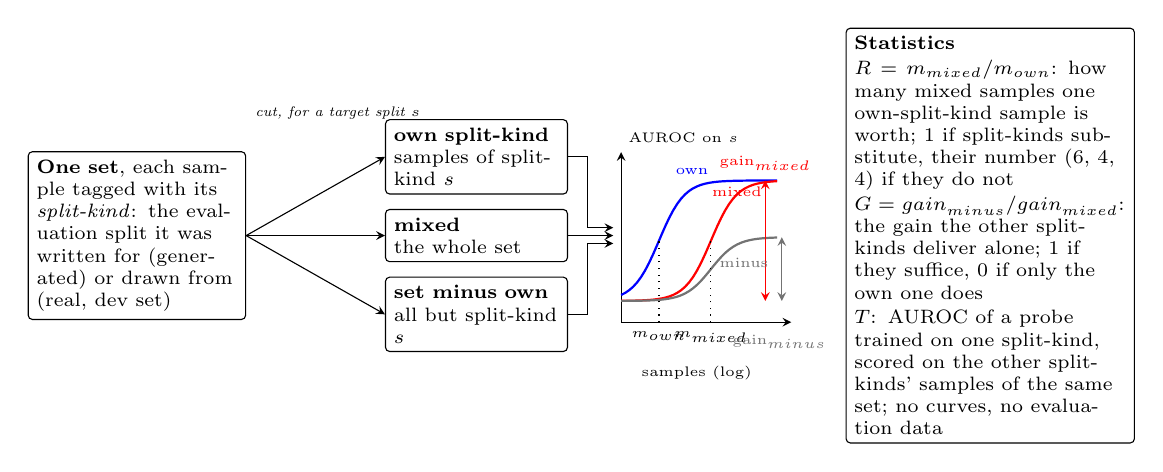
\begin{tikzpicture}[font=\scriptsize, >=stealth,
  box/.style={draw, rounded corners=1.5pt, align=left, inner sep=3pt, text width=#1},
  lab/.style={font=\scriptsize\itshape}]
\node[box=2.55cm] (src) at (0,0) {\textbf{One set}, each sample tagged with its \emph{split-kind}: the evaluation split it was written for (generated) or drawn from (real, dev set)};
\node[box=2.1cm, anchor=west] (kind) at (3.15,1.0) {\textbf{own split-kind}\\ samples of split-kind $s$};
\node[box=2.1cm, anchor=west] (mix)  at (3.15,0.0)  {\textbf{mixed}\\ the whole set};
\node[box=2.1cm, anchor=west] (minus) at (3.15,-1.0) {\textbf{set minus own}\\ all but split-kind $s$};
\draw[->] (src.east) -- (kind.west);
\draw[->] (src.east) -- (mix.west);
\draw[->] (src.east) -- (minus.west);
\node[lab, anchor=south, font=\tiny\itshape] at (2.55,1.35) {cut, for a target split $s$};
% curve sketch
\begin{scope}[shift={(6.15,-1.1)}, x=0.6cm, y=1.8cm]
  \draw[->] (0,0) -- (3.6,0);
  \draw[->] (0,0) -- (0,1.2);
  \node[font=\tiny, anchor=south west] at (-0.05,1.2) {AUROC on $s$};
  \node[font=\tiny, anchor=north] at (1.6,-0.24) {samples (log)};
  \draw[thick, blue] plot[domain=0:3.3, samples=40] (\x, {0.15+0.85/(1+10^(-1.6*(\x-0.8)))});
  \draw[thick, red] plot[domain=0:3.3, samples=40] (\x, {0.15+0.85/(1+10^(-1.6*(\x-1.9)))});
  \draw[thick, black!55] plot[domain=0:3.3, samples=40] (\x, {0.15+0.45/(1+10^(-1.6*(\x-1.9)))});
  \draw[dotted] (0.8,0) -- (0.8,0.575); \node[font=\tiny, below] at (0.8,0) {$m_{\text{own}}$};
  \draw[dotted] (1.9,0) -- (1.9,0.575); \node[font=\tiny, below] at (1.9,0) {$m_{\text{mixed}}$};
  \draw[<->, red] (3.05,0.15) -- (3.05,1.0); \node[font=\tiny, red, above] at (3.05,1.0) {gain$_{\text{mixed}}$};
  \draw[<->, black!55] (3.4,0.15) -- (3.4,0.6); \node[font=\tiny, black!55, below] at (3.35,-0.02) {gain$_{\text{minus}}$};
  \node[font=\tiny, blue] at (1.5,1.06) {own};
  \node[font=\tiny, red] at (2.45,0.92) {mixed};
  \node[font=\tiny, black!55] at (2.6,0.42) {minus};
\end{scope}
\draw[->] (kind.east) -- ++(0.25,0) |- (6.05,0.1);
\draw[->] (mix.east) -- (6.05,0.0);
\draw[->] (minus.east) -- ++(0.25,0) |- (6.05,-0.1);
% statistics
\node[box=3.45cm, anchor=west] (stats) at (9.0,0) {\textbf{Statistics}\\[1pt]
  $R=m_{\text{mixed}}/m_{\text{own}}$: how many mixed samples one own-split-kind sample is worth; 1 if split-kinds substitute, their number (6, 4, 4) if they do not\\[1pt]
  $G=\text{gain}_{\text{minus}}/\text{gain}_{\text{mixed}}$: the gain the other split-kinds deliver alone; 1 if they suffice, 0 if only the own one does\\[1pt]
  $T$: AUROC of a probe trained on one split-kind, scored on the other split-kinds' samples of the same set; no curves, no evaluation data};
\end{tikzpicture}
